\documentclass[11pt]{article}
\usepackage{enumerate}
\usepackage{fullpage}
\usepackage{fancyhdr}
\usepackage{amsmath, amsfonts, amsthm, amssymb}
\usepackage{color}
\usepackage[]{graphicx}

\setlength{\parindent}{0pt}
\setlength{\parskip}{5pt plus 1pt}
\pagestyle{empty}

\def\indented#1{\list{}{}\item[]}
\let\indented=\endlist

\newcounter{questionCounter}
\newcounter{partCounter}[questionCounter]
\newenvironment{question}[2][\arabic{questionCounter}]{%
    \setcounter{partCounter}{0}%
    \vspace{.25in} \hrule \vspace{0.5em}%
        \noindent{\bf #2}%
    \vspace{0.8em} \hrule \vspace{.10in}%
    \addtocounter{questionCounter}{1}%
}{}
\renewenvironment{part}[1][\alph{partCounter}]{%
    \addtocounter{partCounter}{1}%
    \vspace{.10in}%
    \begin{indented}%
       {\bf (#1)} %
}{\end{indented}}

%%%%%%%%%%%%%%%%%%%%%%%HEADER%%%%%%%%%%%%%%%%%%%%%%%%%%%%%%
\newcommand{\myname}{Shashank Singh}
\newcommand{\myandrew}{sss1@andrew.cmu.edu}
\newcommand{\myclass}{86-595 Neural Data Analysis}
\newcommand{\myhwnum}{1}
\newcommand{\duedate}{Tuesday, September 18, 2012}
%%%%%%%%%%%%%%%%%%%%%%%%%%%%%%%%%%%%%%%%%%%%%%%%%%%%%%%%%%%

%%%%%%%%%%%%%%%%%%%%CONTENT MACROS%%%%%%%%%%%%%%%%%%%%%%%%%
\newcommand{\be}{\begin{enumerate}}
\newcommand{\ee}{\end{enumerate}}
\renewcommand{\qed}{\quad $\blacksquare$}
\newcommand{\mqed}{\quad \blacksquare}
\newcommand{\inv}{^{-1}}
\newcommand{\bx}{\mathbf{x}}
\newcommand{\by}{\mathbf{y}}
\newcommand{\bff}{\mathbf{f}}
\newcommand{\bzero}{\mathbf{0}}
\newcommand{\N}{\mathbb{N}} % natural numbers
\newcommand{\Q}{\mathbb{Q}} % rational numbers
\newcommand{\R}{\mathbb{R}} % real numbers
\newcommand{\E}[1]{\mathsf{E}\left[#1\right]} % expected value
\newcommand{\Var}[1]{\mathsf{Var}\left[#1\right]} % variance
\newcommand{\Poisson}[1]{\operatorname{Poisson}\left(#1\right)} % Poisson distribution
\newcommand{\Exp}[1]{\operatorname{Exp}\left(#1\right)} % Exponential distribution
\newcommand{\U}[2]{\operatorname{U}\left(#1,#2\right)} % Uniform distribution
\newcommand{\Bern}[1]{\operatorname{Bernoulli}\left( #1 \right)} % Bernoulli distribution
\newcommand{\pr}[1]{\mathsf{P}\left( #1 \right)} % probability of event #1
\newcommand{\argmax}{\operatorname{argmax}}
%%%%%%%%%%%%%%%%%%%%%%%%%%%%%%%%%%%%%%%%%%%%%%%%%%%%%%%%%%%

\begin{document}
\thispagestyle{plain}

{\Large Homework \myhwnum} \\
\myclass \\
Name: \myname \\
Email: \myandrew \\
Due: \duedate \\
\begin{question}{Problem 1}
By given definition of mutual information,
\begin{align*}
MI(X,Y;S)
 & = \sum_{(x,y) \in X \times Y} \sum_{s \in S}
             p(x,y,s) \log_2 \left( \frac{p(x,y,s)}
                                         {p(x,y)p(s)} \right) \\
 & = \sum_{x \in X} \sum_{y \in Y} \sum_{s \in S}
             p(x,y,s) \log_2 \left( \frac{p(y,s | x)p(x)p(s | x)}
                                         {p(y | x)p(x)p(s)p(s | x)} \right) \\
 & = \sum_{x \in X} \sum_{y \in Y} \sum_{s \in S}
             p(x,y,s) \left( \log_2 \left( \frac{p(x,s)}
                                         {p(x)p(s)} \right) + \log_2 \left( \frac{p(y,s | x)}{p(y | s)p(s | x)} \right)\right)\\
 & = \sum_{x \in X} \sum_{y \in Y} \sum_{s \in S}
             p(x,y,s) \log_2 \left( \frac{p(x,s)}
                                         {p(x)p(s)} \right)
   + \sum_{x \in X} \sum_{y \in Y} \sum_{s \in S}
             p(y,s | x)p(x) \log_2 \left( \frac{p(y,s | x)}{p(y | s)p(s | x)} \right)\\
 & = \sum_{x \in X} \sum_{s \in S}
             p(x,s) \log_2 \left( \frac{p(x,s)}
                                         {p(x)p(s)} \right)
   + \sum_{x \in X} p(x) \sum_{y \in Y} \sum_{s \in S}
             p(y,s | x)p(x) \log_2 \left( \frac{p(y,s | x)}{p(y | s)p(s | x)} \right)\\
 & = MI(X;S) + MI(Y;S | X). \mqed
\end{align*}
\end{question}

\begin{question}{Problem 2}
By definition of entropy,
\begin{align*}
H(Y)
 & = -\sum_{n = 0}^{\infty} p(y = n) \log(p(y = n))
   = -\sum_{n = 0}^{\infty} \frac{\lambda^n}{n!}e^{-\lambda} \log \left(\frac{\lambda^n}{n!}e^{-\lambda} \right)
 & \left( p(Y = n) = \frac{\lambda^n}{n!}e^{-\lambda} \right) \\
 & =  \sum_{n = 0}^{\infty} \frac{\lambda^n}{n!}e^{-\lambda} \left( -\log(\lambda^n) - \log(e^{-\lambda}) + \log(n!) \right) \\
 & = - \lambda\log(\lambda)\sum_{n = 1}^{\infty} \frac{\lambda^{n - 1}}{(n - 1)!}e^{-\lambda}  
     + \lambda             \sum_{n = 0}^{\infty} \frac{\lambda^n}{n!}e^{-\lambda}
     +                     \sum_{n = 0}^{\infty} \frac{\lambda^n}{n!}e^{-\lambda} \log(n!) \\
 & = \lambda(1 - \log(\lambda))
     + e^{-\lambda} \sum_{n = 0}^{\infty} \frac{\log(n!)\lambda^n}{n!}. \mqed
 & \left(\sum_{n = 0}^{\infty} \frac{\lambda^n}{n!}e^{-\lambda} = 1\right)
\end{align*}
\end{question}

\newpage
\begin{question}{Problem 3}
\begin{enumerate}[a.]
\item Note that $P(Y = 0) = \dots = P(Y = 4) = 0.2$. Thus, by Problem 4a.,
$H(Y) = \log_2(5)$.

\item
\begin{align*}
MI(T;Y) 
 & = \sum_{t = 1,2} \sum_{y = 0,1,2,3,4} p(T = t,Y = y) \log_2 \left( \frac{p(T = t,Y = y)}{p(T = y)p(Y = y)} \right) \\
 & = \sum_{t = 1,2} \sum_{y = 0,1,2,3,4} p(T = t,Y = y) \log_2 \left( \frac{p(T = t,Y = y)}{(0.5)(0.2)} \right)
\end{align*}

\end{enumerate}
\end{question}

\begin{question}{Problem 4}
\begin{enumerate}[a.]
\item By definition of entropy,
\[H(X)
 = -\sum_{x \in X} \frac{1}{N} \log_2\left( \frac{1}{N} \right)
 = -N\frac{1}{N} \log_2\left( \frac{1}{N} \right)
 = \log_2(N). \mqed
\]

\item Suppose $p: X \rightarrow \R$ is a probability distribution on some
finite set $X$, and suppose $q$ is the uniform distribution on $X$.
Then, by definition of entropy,
\begin{align*}
0 \leq D(p || q)
 & = \sum_{x \in X} p(x) \log_2\left( \frac{p(x)}{q(x)} \right)
   = \sum_{x \in X} p(x) \log_2\left( \frac{p(x)}{1/|X|} \right)        \\
 & = \sum_{x \in X} p(x) \left( \log_2(p(x)) + \log(|X|) \right)        \\
 & = \log_2(|X|)\sum_{x \in X} p(x) + \sum_{x \in X} p(x) \log_2(p(x))
   = \log_2(|X|) - H(p).
\end{align*}

Thus, $D(p || q)$ is minimized when $H(p)$ is maximized.
Since $D(p || q) \geq 0$, with equality holding if and only if $p = q$ on
$X$, $D(p || q)$ is minimized (so that $H(p)$ is maximized) when $p = q$. \qed
\end{enumerate}
\end{question}

%TODO
\begin{question}{Problem 5}
\begin{enumerate}[a.]
\item By the result of part a. of problem 4, $H(S) = \log_2(4) = \mbox{\fbox{$2$.}}$

\item
\begin{tabular}{|c|c|c|c|c|}
\hline
$\theta$                    & $0^{\circ}$ & $45^{\circ}$ & $90^{\circ}$ & $135^{\circ}$ \\
\hline
$H(R | S = \lambda_\theta)$ & 27.45       & 7094.62      & 869114.22    & 78436652.48   \\
\hline
\end{tabular}

The above values were computed by the following MATLAB code:
\begin{verbatim}
>> L = (2:2:8)';
>> N = 1:15;
>> for j=1:15, S(:,j) = gammaln(j).*(L.^(N(j)))./factorial(j); end
>> H = L.*(1 - log(L)) + exp(L).*sum(S,2);
\end{verbatim}


\item
\[H(R | S)
 = \frac14 \sum_{s \in S} H(R | S = s)
 = \mbox{\fbox{$19828222.19$.}}\]

\item

\item $MI(R;S) = H(R) - H(R | S)$

\item 
\begin{figure}[h]
\begin{center}
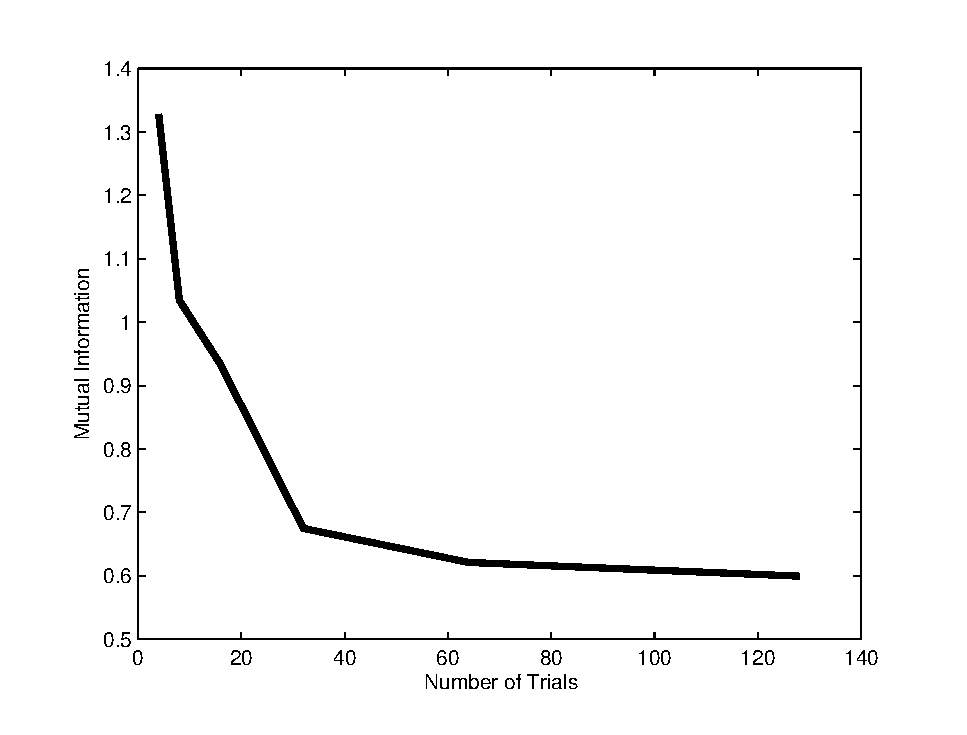
\includegraphics[width=0.46\textwidth]{5f}
\end{center}
\label{fig:5f}
\end{figure}

\item
\begin{figure}[h]
\begin{center}
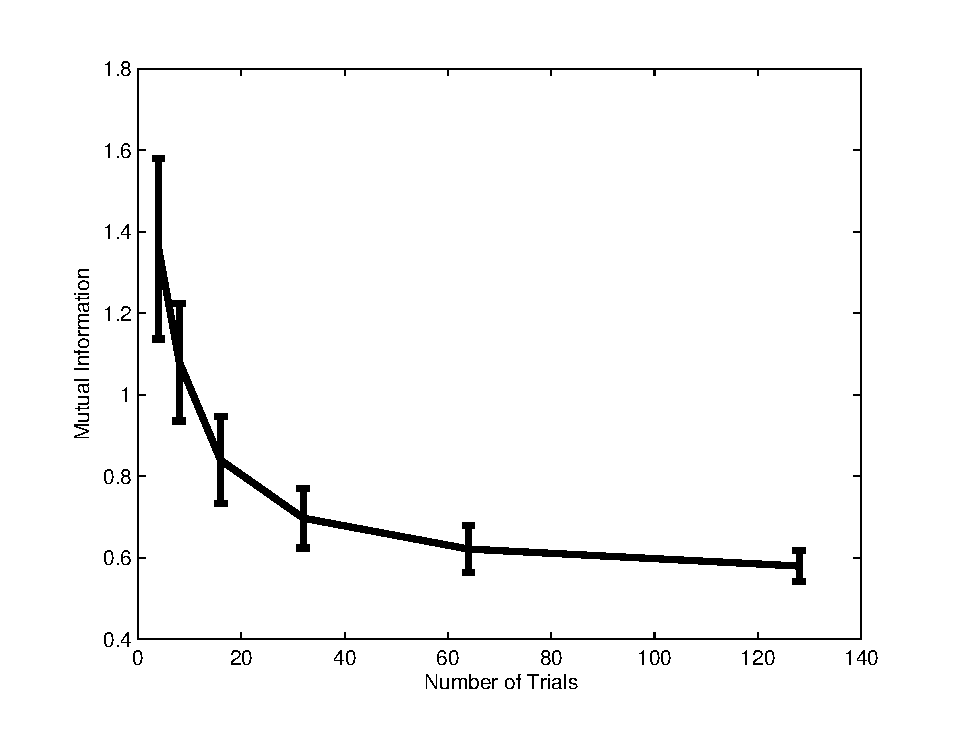
\includegraphics[width=0.46\textwidth]{5g}
\end{center}
\label{fig:5g}
\end{figure}

\item Both the mean and standard deviation in estimated mutual information
decrease as the number of trials increases, sharply at first, and then more
gradually.

%TODO
\item

%TODO
\item

\end{enumerate}
\end{question}

\begin{question}{Problem 6}
The simulation took me quite a while this time, and I'm not sure I understand,
theoretically, why data insufficiency causes mutual information to be
overestimated. 1,2, and 4 were easy enough (4b. was especially nifty), but 3
involved a lot of calculation. The math for information theory seems really
ugly\dots
\end{question}

The following MATLAB code was used to empirically compute mutual information
for problem 5:

\begin{verbatim}
MI = zeros(100,6);

for trial=1:100
  num = 1;
  for N=[4 8 16 32 64 128];
    data = [poissrnd(2,1,N);
            poissrnd(4,1,N);
            poissrnd(6,1,N);
            poissrnd(8,1,N)];

    for i=1:4
      u = unique(data(i,:));
      prob{i} = zeros(2,length(u));
      prob{i}(1,:) = u;
  
      for j=1:length(u)
        prob{i}(2,j) = length(find(data(i,:) == prob{i}(1,j)))./(4*N);
      end
    end
  
    all = [prob{1} prob{2} prob{3} prob{4}];
    u = unique(all(1,:));
    pr = zeros(2,length(u));
    pr(1,:) = u;
  
    for i=1:length(u)
      pr(2,i) = sum(all(2,find(all(1,:) == pr(1,i))));
    end
  
    HR = -sum(pr(2,:).*log2(pr(2,:)));
    HRS = -sum(all(2,:).*log2(4.*all(2,:)));
    MI(trial,num) = HR - HRS;

    num = num + 1;
  end
end
\end{verbatim}
\end{document}
